\chapter{Analysis of spatial-diversity with a numerical simulator}
The previous chapter introduced the idea of exploiting spatial-diversity to provide more priority levels for flow classification. It was discussed why in principle such technique could yield flow completion time gains, especially when few priority queues are available. It was explained that adopting a spatial-diversity demotion has strong implication on the traffic load balancing, since flow routing becomes priority-dependent.  A few questions arises soon: how to choose the thresholds to distribute the load on the topology? What are the relationships between the priority granularity in 
single interfaces and spatial diversity? Is the best choice to use all spines for incremental priorities when the topology is big? The goal of this chapter is to validate these intuitive hints with numerical results and to shed the light on the benefits and the restraints of the proposed algorithm. In particular, it will go through an exhaustive analysis of the system by delivering plenty of numerical experiments obtained with a custom flow simulator implemented in Python. This simulator does not capture any of the complex dynamics inherent to a real packet network, it does not have any protocol stack implemented neither at traffic sources modules nor in the switching modules. Rather, it is a job-oriented queueing simulator that does not care about packets but only runs flow arrivals and serve them in queuing modules. Its purpose is to provide a clean baseline numerical analysis not plagued by possible side effects due to network misconfiguration.
\section{Spatial-diversity framework}

\subsection{Problem abstraction}
To tackle spatial-diversity in the initial phase and get a first glance about its effectiveness, three queuing systems are compared. They are shown in Fig.\ref{fig:three-system-comparison}. 

\begin{figure}
	\centering
	\begin{subfigure}[b]{0.3\textwidth}
		\centering
		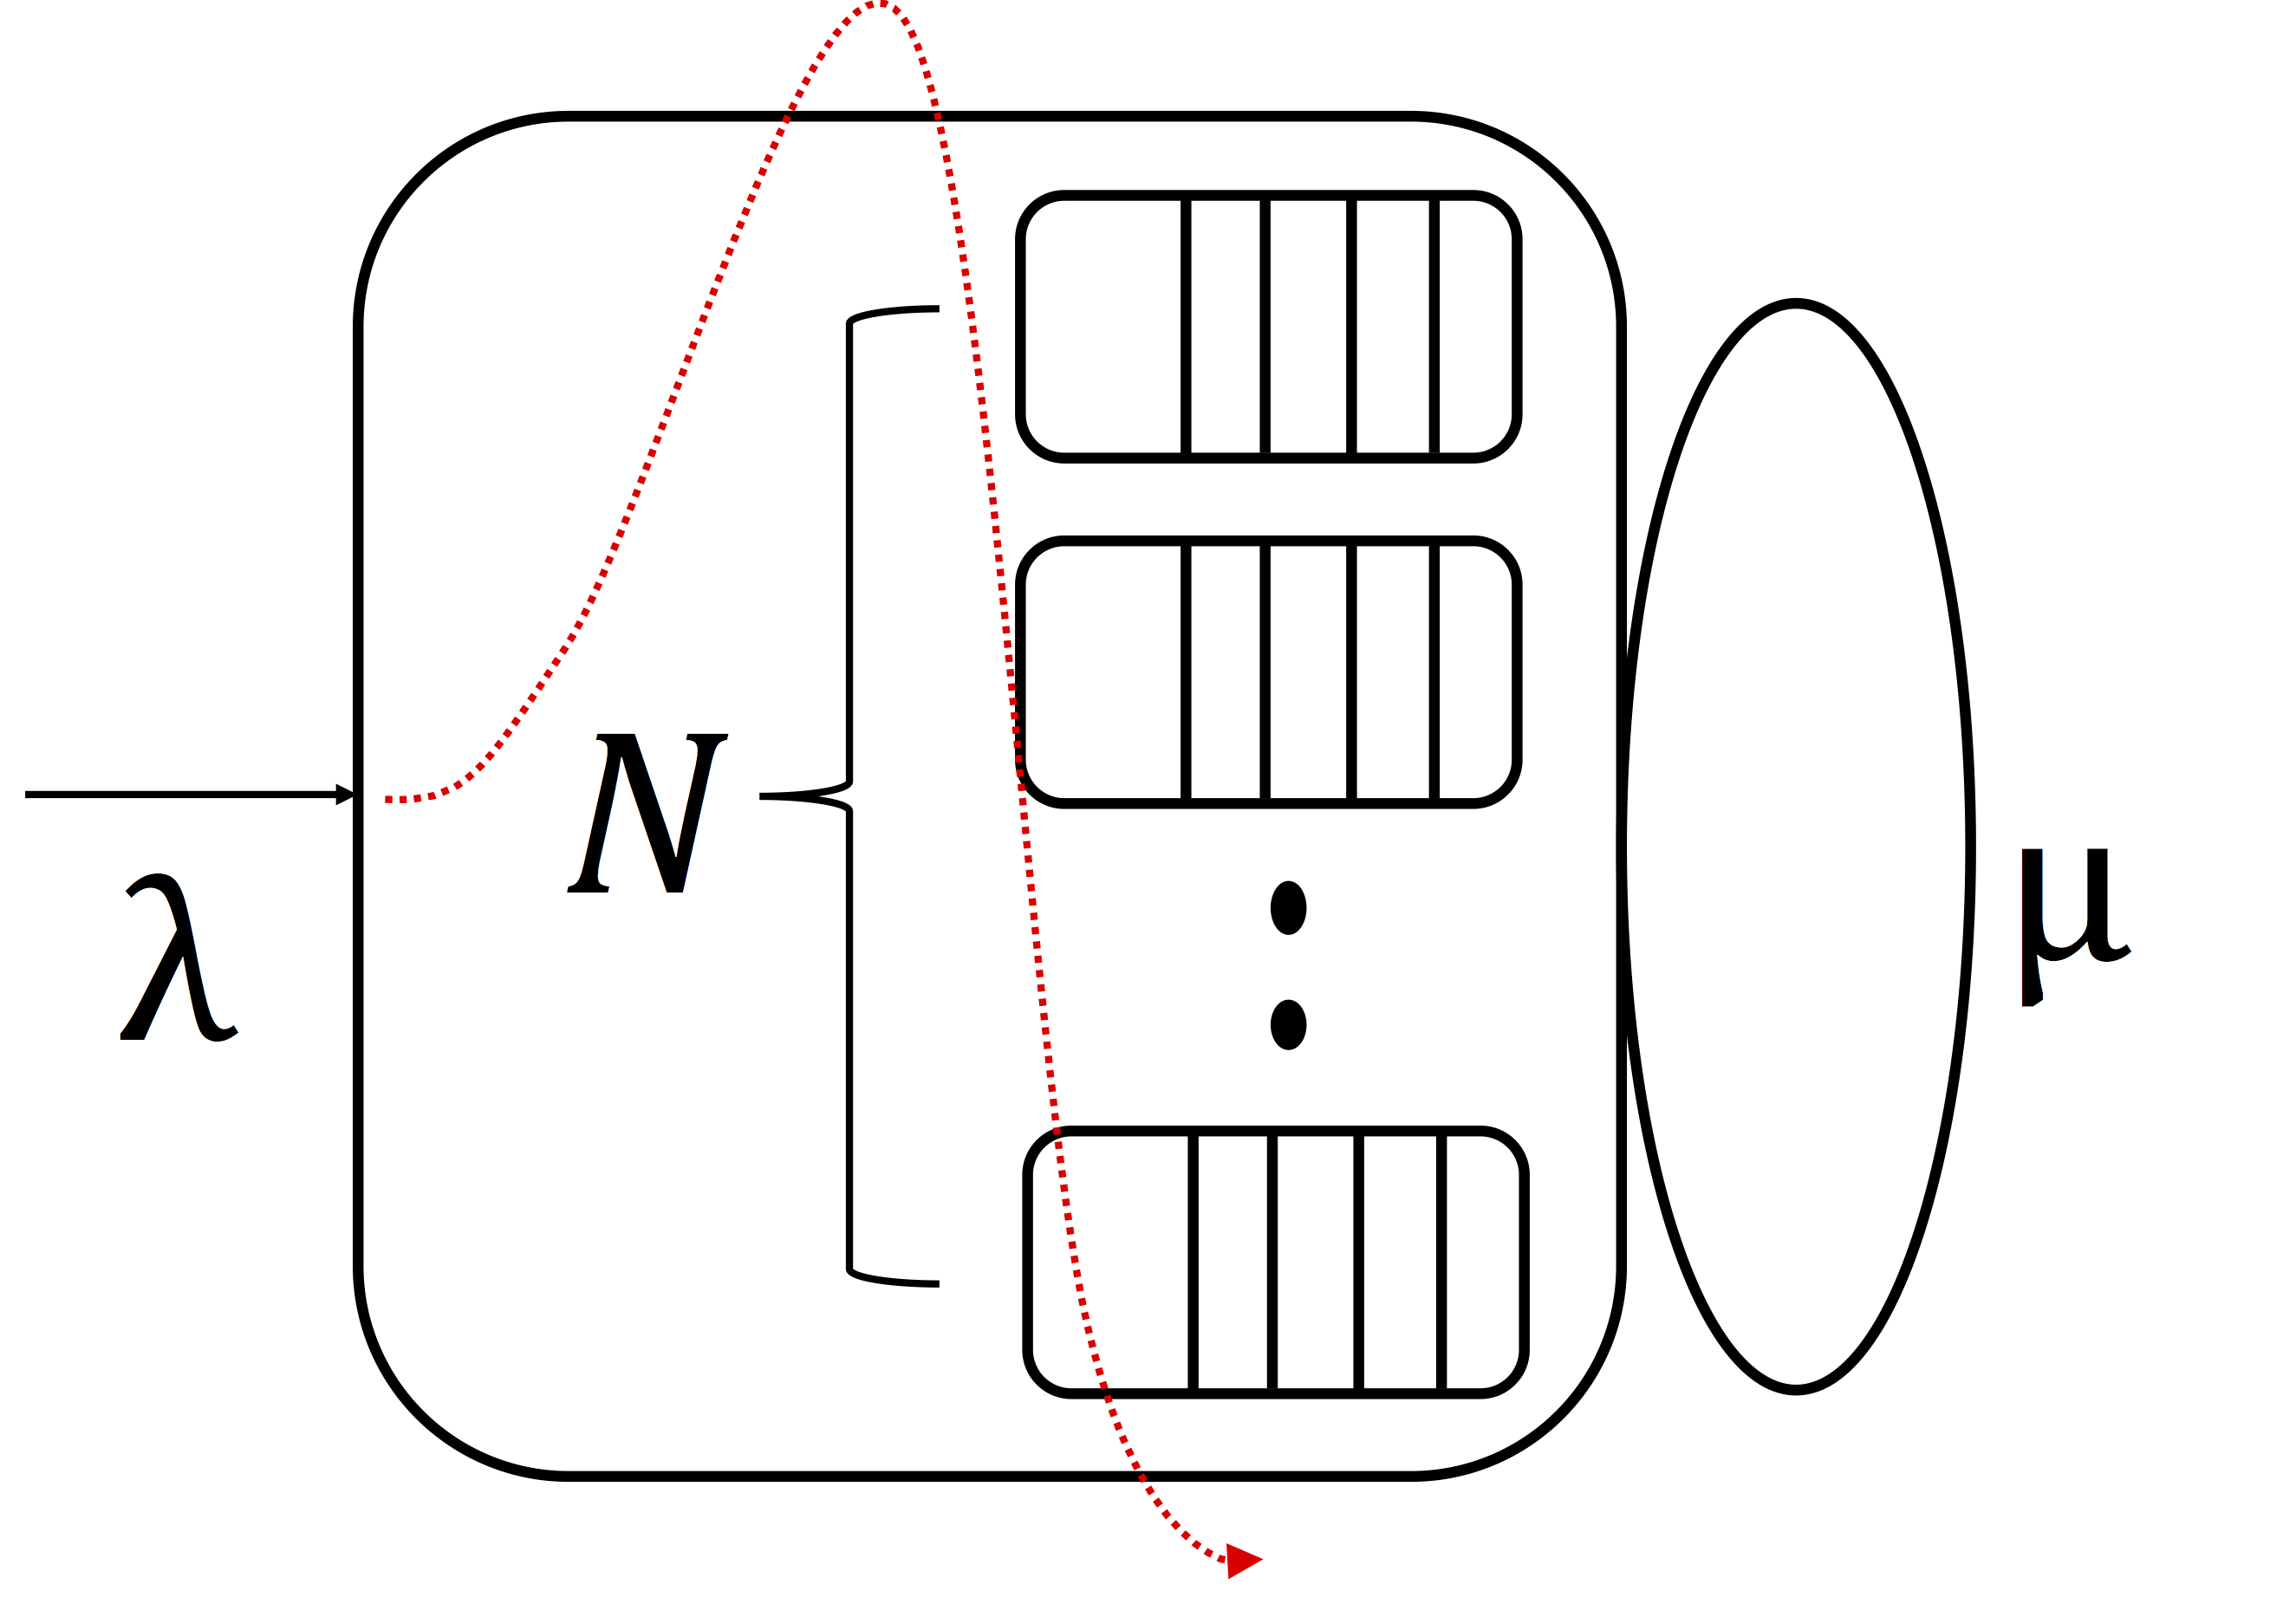
\includegraphics[width=\textwidth]{Chapter3/Figures/switchone}
		\smallskip
		\caption{Super-Server}
		\label{fig:switchone}
	\end{subfigure}
	\hfill
	\begin{subfigure}[b]{0.3\textwidth}
		\centering
		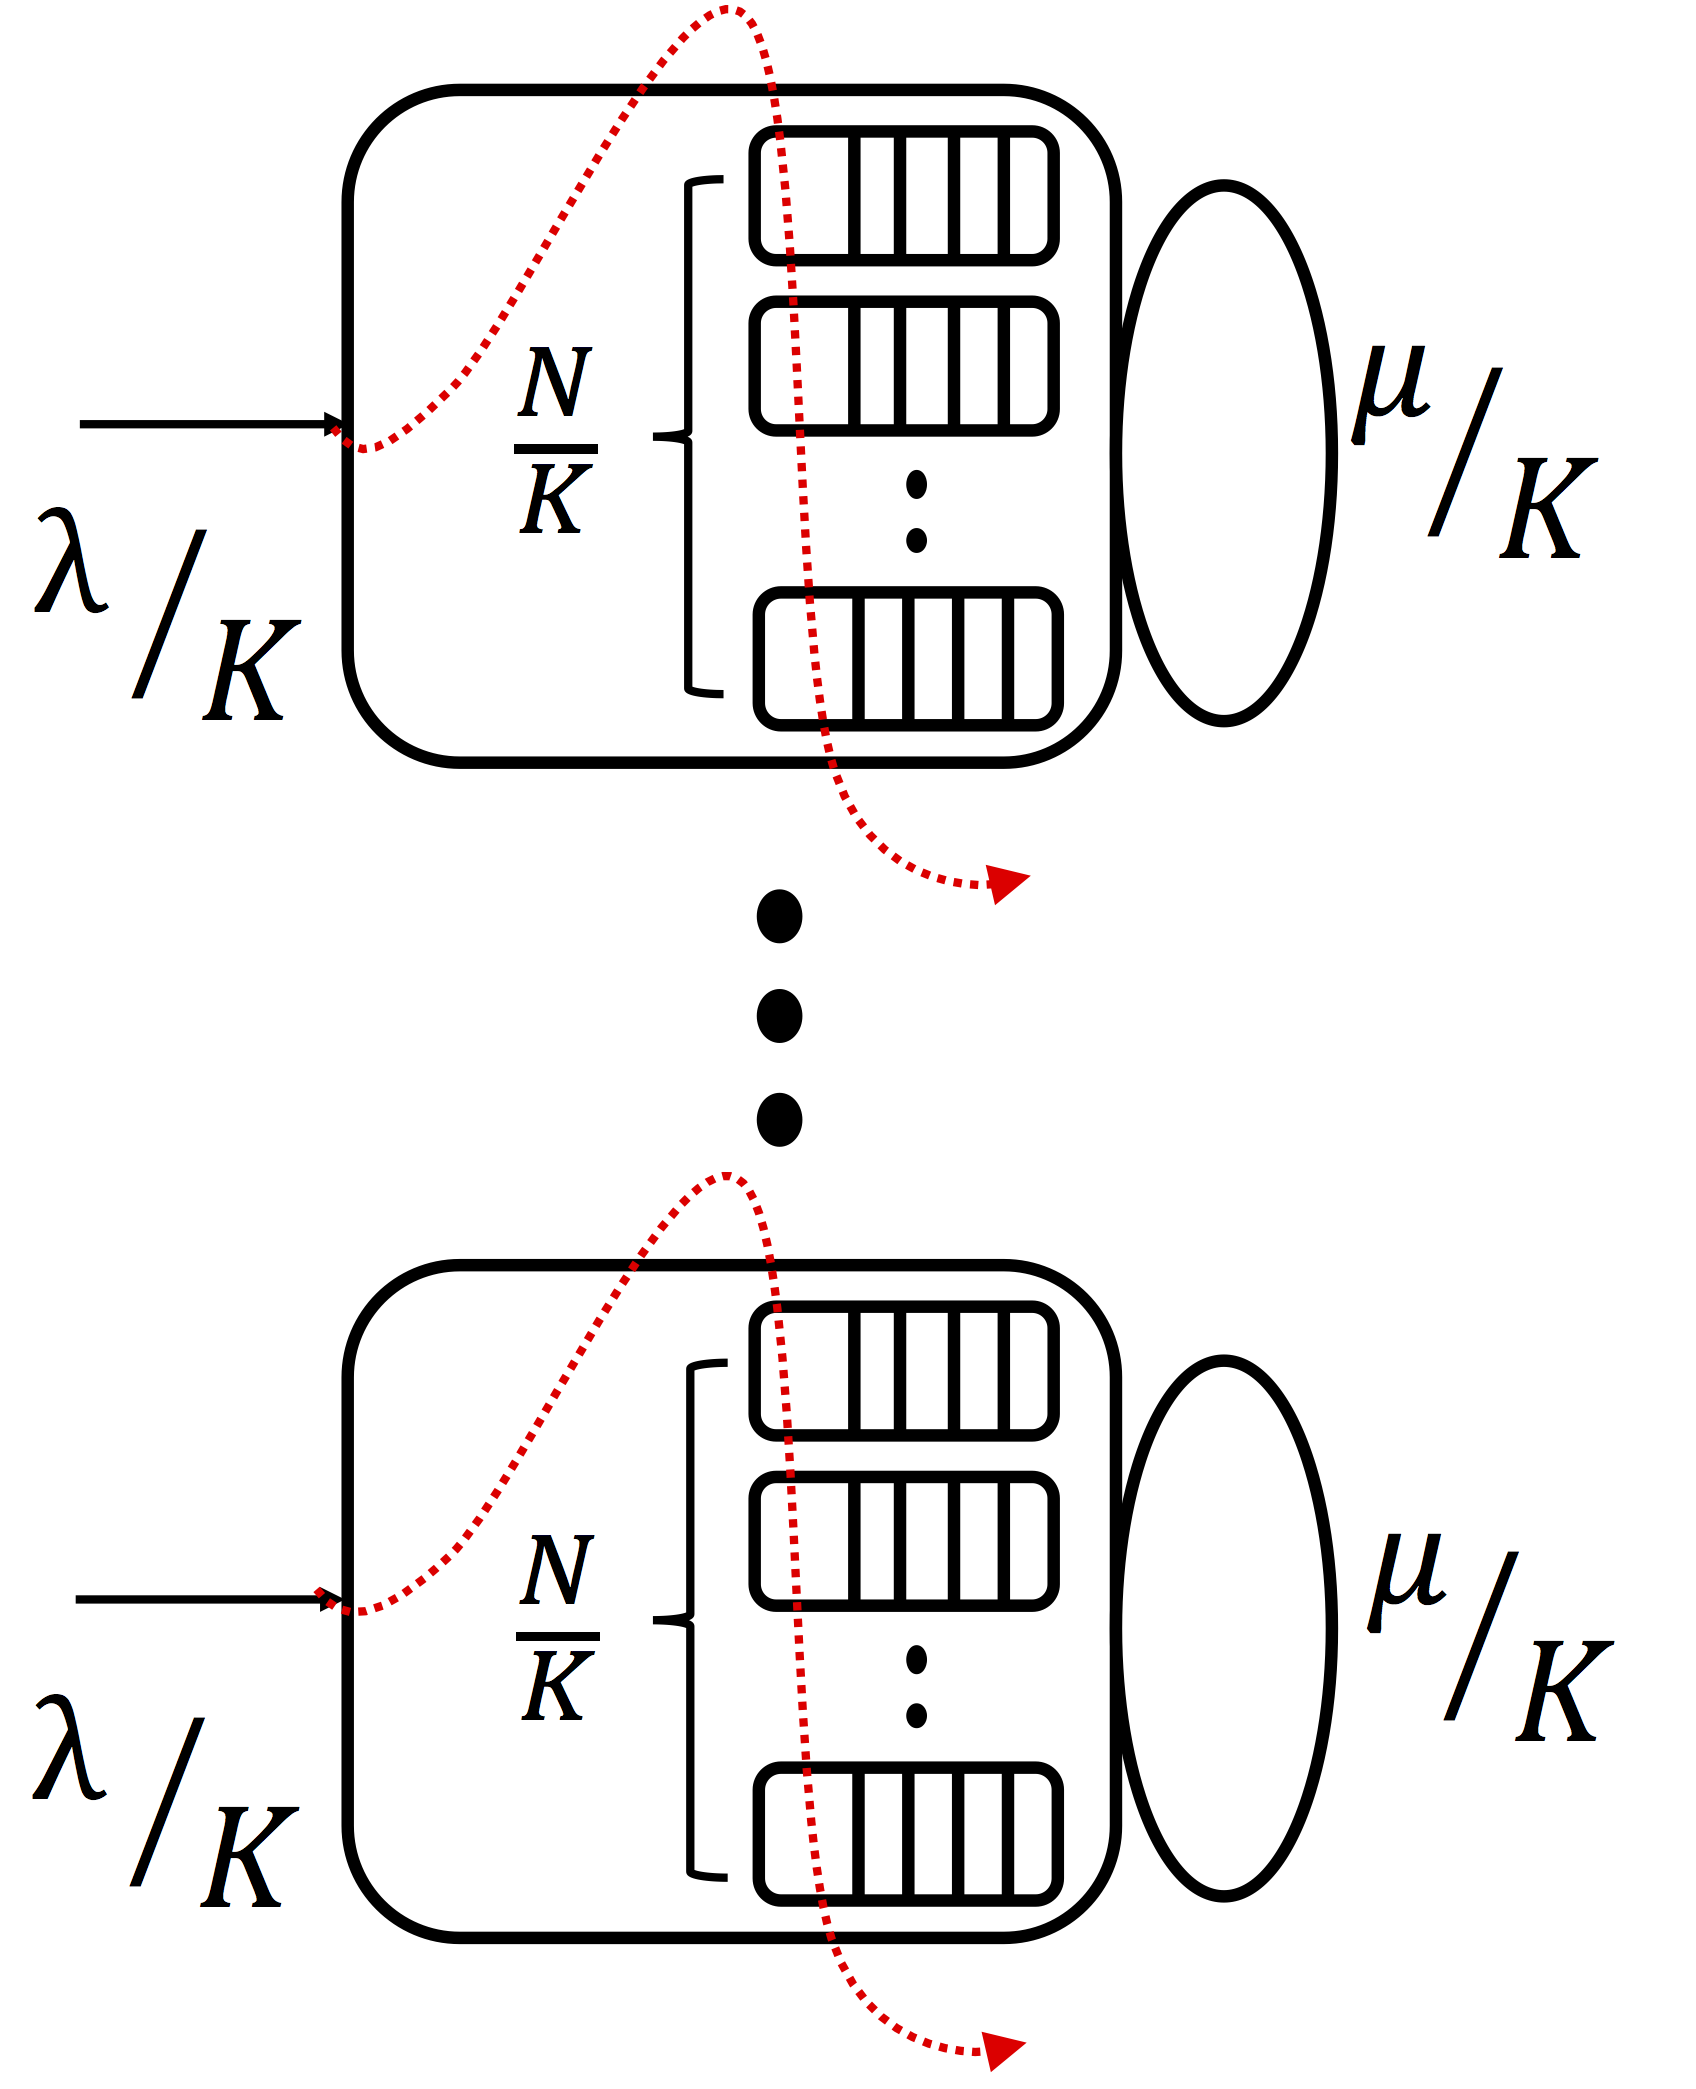
\includegraphics[width=0.8\textwidth]{Chapter3/Figures/esn}
		\caption{Independent servers}
		\label{fig:enn}
	\end{subfigure}
	\hfill
	\begin{subfigure}[b]{0.3\textwidth}
		\centering
		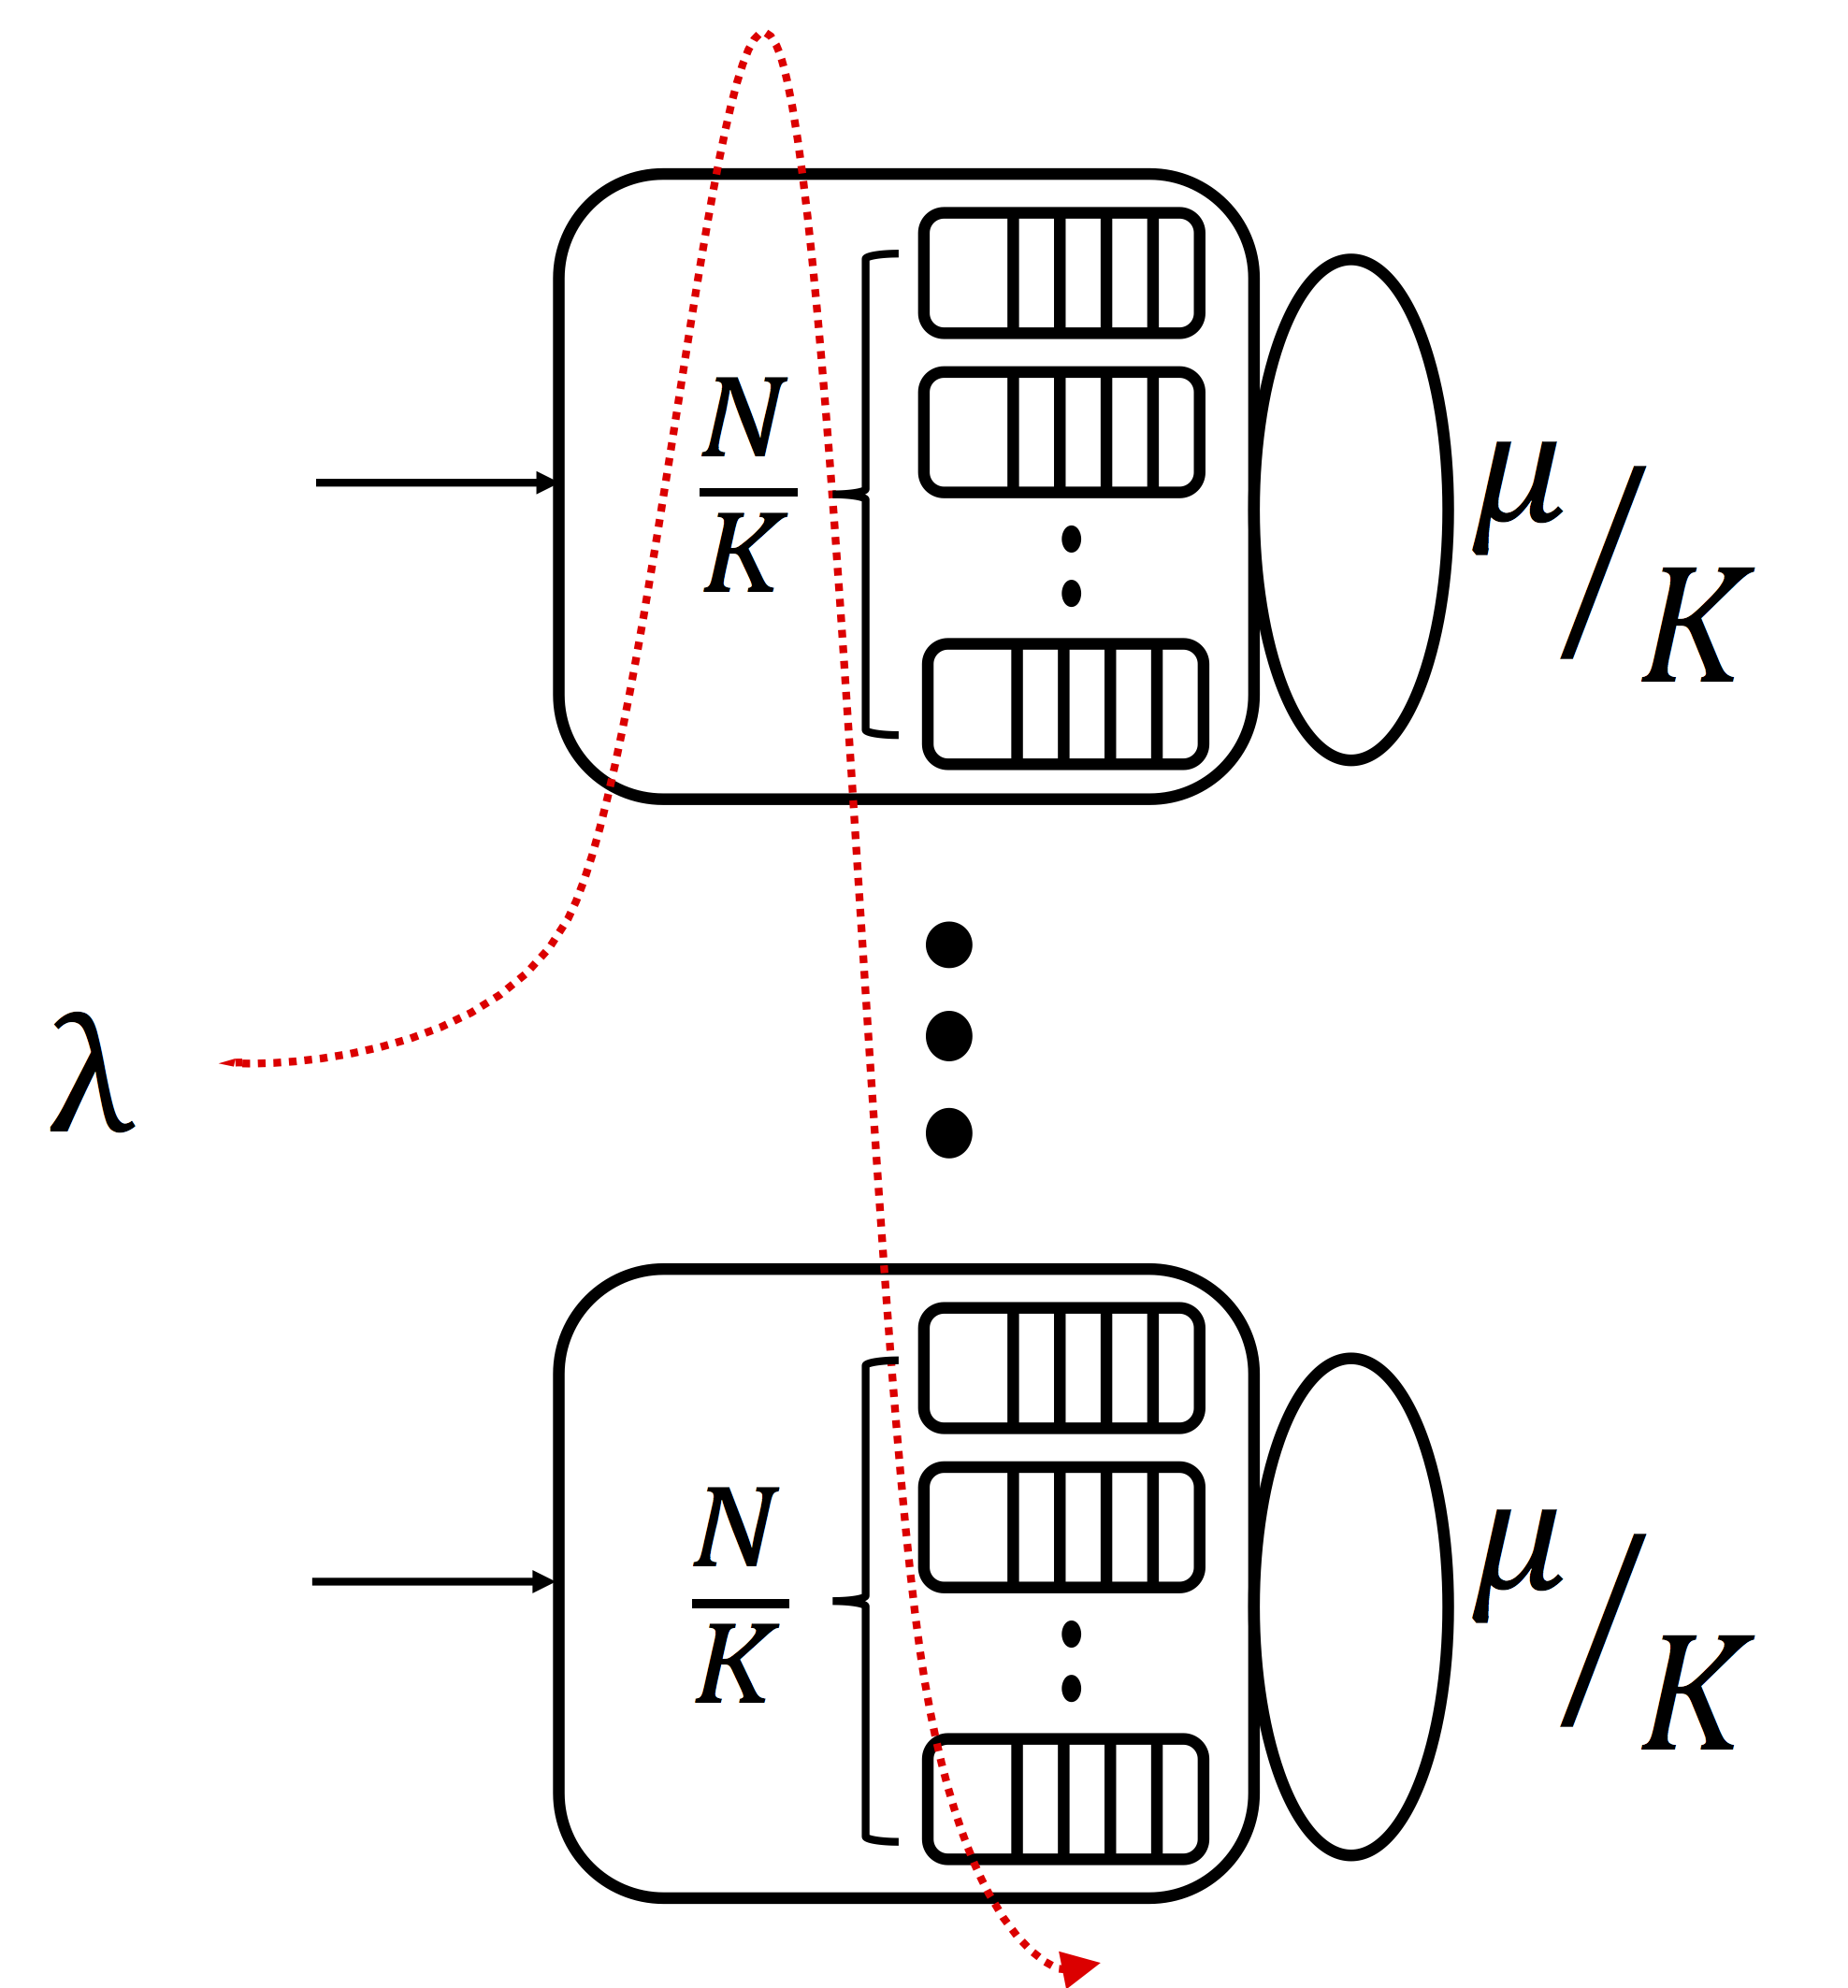
\includegraphics[width=0.9\textwidth]{Chapter3/Figures/sdmlfq}
		\caption{Spatial-diversity}
		\label{fig:sdmlfq}
	\end{subfigure}
	\caption{Three queuing system comparison.} %Red arrows indicate how queues are traversed during flow demotion. On each switch is reported the number of priorities it handles. Color scale is used to emphasize priority levels.}
	\label{fig:three-system-comparison}
\end{figure}

This is a general abstraction of the real system in a datacenter topology. At its heart, actually, a Leaf-and-Spine network with $K$ spines can be described with a scheme of $K$ parallel servers. These servers can be equivalently mapped to the \textit{up-send} interfaces that connects a ToR switch to all the spines, as well as to the \textit{down-send} interfaces that from different spines forward the traffic to a single ToR. Ingress and egress ports that connect end hosts to the datacenter network are ignored at this stage. This is in contrast with the data center abstraction of pFabric as a giant switch presented previously (Figure \ref{fig:pfabricdcn}), where the ingress and egress queues were the bottleneck links where to deploy best scheduling strategies. Also PIAS, optimizing its thresholds on the bottleneck link embraced a similar model. Somehow, differently from the state-of-the-art solutions that focus only on the bottleneck link assuming that with no oversubscription and ideal load balancing the network is able to sustain maximum throughput with negligible delays, the spatial-diversity approach shifts the attention on the queues inside the fabric itself. The integration with ingress and egress queues will be managed afterwards.\\
From now on and for the rest of this section, the interfaces abstracted in the simplified queuing model will be referred to as servers. The three systems are compared on the same conditions of total arrival rate $\lambda$, processing power $\mu$ and priority levels $N$, but with different partitioning of the same priority levels on a number $K$ of servers and, more importantly, with different demotion trajectories. Specifically, all systems use priority demotion first introduced by PIAS (\S \ref{sec:pias}). Red arrows indicate the trajectory across all available priority queues followed by the longest flow that experience the maximum number of demotions. \\
The first case (Fig. \ref{fig:switchone}) is to have a single high-capacity server that handles all priorities. This of course is the absolute best case where resources are fully concentrated, that doesn't exist in real systems and that provides the smallest delay. It would be equivalent to realize an entire data center interconnection network with a single device of astonishing bandwidth. The second case (Fig. \ref{fig:enn}) is the legacy way to handle priority demotion, where all servers are treated independently in parallel. Flows are evenly load balanced on the available servers and moved across priorities of the same server during their lifetime. In this case the number of demotion levels are limited to \small$\frac{N}{K}$\normalsize. Finally, the third case (Fig. \ref{fig:sdmlfq}) is the novel object under investigation, where all the flows are initially sent to the same server, then demoted on the $N$ globally available priority queues. In this case subsequent servers are configured to handle lower and lower priorities, thus part of the flows are re-routed as a consequence of the spatial-diversity. In the following, also the servers and the links may be labeled as "high priority" or "low priority" for brevity, meaning that they handle high priority traffic or low priority traffic, respectively. 

\subsection{Workloads}
The performances of the three systems are compared using two empirical flow size distributions that have been derived from production data centers (Figure \ref{fig:workloads}). Flow size distribution is shortly termed \emph{workload}. The first workload has been estimated instrumenting thousands of servers in a datacenter hosting a Web search \cite{dctcp} application, while the other refers to data mining tasks \cite{vl2}. 
\begin{figure}
	\centering
	\begin{subfigure}[b]{0.49\textwidth}
		\centering
		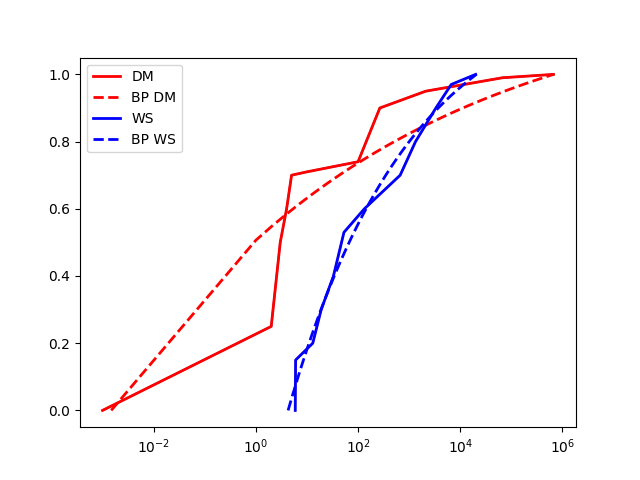
\includegraphics[width=\textwidth]{Chapter3/Figures/fits}
		\caption{CDF}
		\label{fig:cdfs}
	\end{subfigure}
   \hfill
   \begin{subfigure}[b]{0.49\textwidth}
   	\centering
   	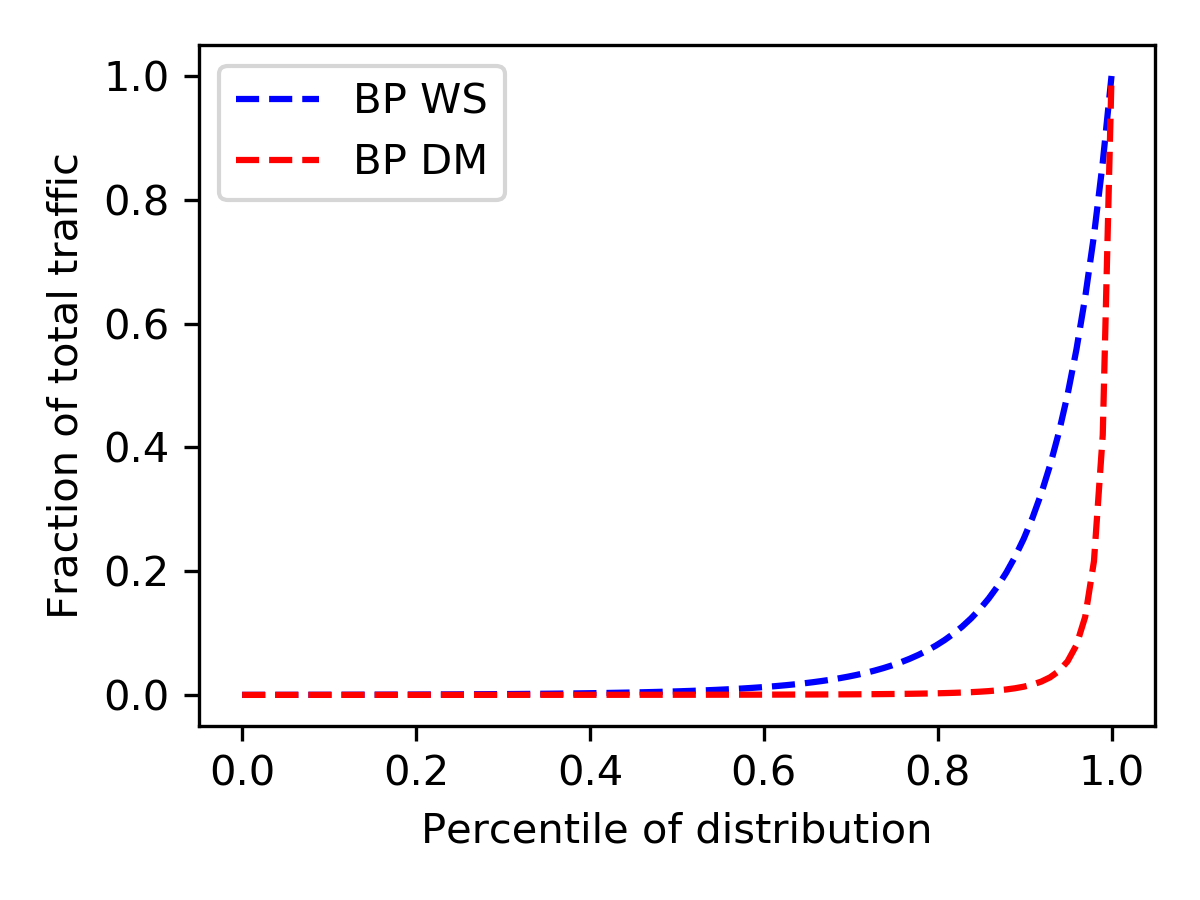
\includegraphics[width=\textwidth]{Chapter3/Figures/mwf}
   	\caption{MWF}
   	\label{fig:mwf}
   \end{subfigure}
	\caption{Workload properties}
	\label{fig:workloads}
\end{figure}
As expected, these distributions have a mix of short and long flows and both present the high-variability property typical of data center traffic (\S \ref{sec:traffic-properties}). Figure \ref{fig:cdfs} shows with solid lines the cumulative density function of the two empirical workloads, along with two dashed Bounded Pareto distributions, whose parameters have been fitted to the corresponding empirical points. The bounded Pareto distribution is a truncated version of the Pareto distribution over the finite support $[u,t]$ and it is well-suited to model heavy-tail characteristics. It has three parameter: the lower extreme of its support $u$, the upper extreme $t$ and the shape parameter $\alpha$ that controls the weight of its tail. The analytical expression of its cdf $F(x)$ in the interval $[u,t]$ is:
\begin{equation}
	F(x) = \dfrac{1-\Big(\dfrac{u}{x}\Big)^{\alpha}}{1-\Big(\dfrac{u}{t}\Big)^{\alpha}}, \qquad 0 \le \alpha \le 2
\end{equation}
This distribution has been chosen to be used in the analysis due to some graceful properties. First of all, it is relatively easy to control its variability by a proper tuning of its parameter $\alpha$. Values of $\alpha$ close to 2 accentuate the heavy-tail property, while smaller values of $\alpha$ tend to regularize a bit its behavior. Second, being definite on a limited support it can be adapted to any minimum and maximum flow size in the datacenter. Last, its mean and its variance  --- which depend on $\alpha$ --- are finite, thus the problem of finding the shape parameter for any fixed first and second moment can be smoothly treated numerically. Specifically, for the bounded Pareto, the mean and the variance have the following expression:
\begin{align*}
\mathbb{E}[X] &= \dfrac{\alpha}{(1-\alpha)(t^{\alpha}-u^{\alpha})} (u^{\alpha}t - t^{\alpha}u) \\ \\
\sigma_X^2 &= \dfrac{\alpha}{(2-\alpha)(t^{\alpha}-u^{\alpha})} (u^{\alpha}t^2 - t^{\alpha}u^2)
\end{align*}
The best fit to the empirical distributions has been obtained with a simple Maximum Likelihood Estimator (MLE). The resulting parameters are reported for both the workloads. Let $X$ be the flow size random variable as usual, and write in short notation \textit{BP}($u,t,\alpha$) the bounded Pareto. 
\begin{align*}
	X_{WS} \sim& \text{\textit{BP}}(3, \, 29000, \, 0.125)\\
	X_{DM} \sim& \text{\textit{BP}}(0.1, \, 100000, \,0.26)
\end{align*}
The measurement unit for the extremes of the support in this case is kilobytes. The fitting error is higher for the data mining workload than for the web search. For low percentiles this is difficult to avoid because a very crude sampling is provided. In fact, on a total of 11 empirical points, 4 of them are for values above the 90th percentile. Instead, for high percentiles a better fitting likely could be obtained by weighting more the tail of the distribution. However, since the simulations will be performed with the empirical traces, this point is neglected. \\
The rightmost plot (Fig. \ref{fig:mwf}) completes the picture by showing the Mass-Weighted Function $M_w(x)$ \cite{mwf}. This can be seen as the probability that a byte picked at random belongs to a flow below a given percentile and it is used to characterize the variability of a distribution. Its name comes from its definition, where job sizes are weighted by their probability mass:
\[
M_w(x) = \dfrac{\int_{0}^{x} x f(x) dx}{\mathbb{E}[X]}
\]
It holds:
\[
\int\nolimits_{0}^{x} x f(x) dx \le \mathbb{E}[X]
\]
In other words, it is just the average normalized traffic injected by flows shorter than $x$. The figure has on the abscissa the percentile rather than the corresponding job size, to allow the comparison between workloads with different supports on the same axis. If $y$ is a given percentile, it is evaluated $M_w(F^{-1}(y))$. \\
In summary, both distributions exhibit high variability. In the web search case the largest 4\% of flows carry half of the total traffic, the data mining is even more skewed: 70\% of the flows are less than 8 packets only, but almost the entire load is sustained by a ridiculous percentage of flows of about 100MB of size. This suggests that the more challenging distribution to schedule is the web search, consequently it is the one that will deserve most of the attention. In fact, recall that an ideal flow-agnostic LAS scheduler guarantees lower and lower delays as the variability of the distribution increases, both on average and at high percentiles (\S \ref{sec:las}). The theory is confirmed pretty straightforwardly by the simulation results presented next. Moreover, the web search distribution is also a lot easier to simulate, since the very long tails of the data mining workload require protracted time-consuming simulations before being precisely reproduced. Long flows occur sporadically, however they give the main contribution to generate a desired load on the system. 

\subsection{Optimal traffic load balancing}
In previous discussions, it was already realized that the spatial diversity framework introduces strong implications on how the load is distributed on the switching fabric, in particular on the bisection bandwidth. To clarify the concept let's come back to the abstract model considered so far and let's analyze the simpler example of spatial diversity, where only two M/M/1 servers are deployed in parallel, each of them with only a single priority queue. With this setup all flow demotions correspond to shifting a flow from one server to the other. Therefore, the assignment of the demotion threshold can be equivalently seen as a load balance problem. If the threshold is too small, flows are early rerouted on the low priority path and the capacity of the high priority link is essentially wasted. For the real data center implementation this would mean a 50\% throughput reduction of the switching fabric. On the other end, the traditional \textit{perfect} load balance which uniformly splits the traffic on available servers may correspond to a bad demotion threshold for the FCT minimization. Depending on the shape of the flow size distribution, latency constrained traffic would remain unnecessarily mixed with non-demanding latency flows. Certainly, the same issues arise the same augmenting the dimensionality of the topology and the priority queues. 
A careful tuning of load balance is a new trade-off that was nonexistent in the legacy MLFQ framework, where traffic was demoted to different priority queues but still in the same interface (i.e. link). If that is the case, a threshold setting that gives an unbalanced load allocation in the available priority queues affects only the delays but not the maximum throughput that the network can sustain. The introduction of spatial diversity adds a level of complexity to the system. 

Two related problems need to be solved: finding the set of thresholds that triggers a new flow route from one server to another and finding for each server a set of thresholds that mark the demotion boundaries among PQs. Let's denote them as \emph{load-balance thresholds} and \emph{sub-thresholds} respectively.
In section \ref{sec:complete-model} was presented an extension to the PIAS model that embeds spatial-diversity. This formulation would in principle address both problems. In fact, the optimal solution would never include load balance thresholds that overload some servers, because that would overkill the delays which the problem tries to minimize. At the same time, a unique formulation would choose a set of sub-thresholds targeted on the optimal load balance thresholds, providing a joint solution.  Despite being a clean analytical formulation, its complexity seems prohibitive. The basic model without spatial diversity yet was non-convex and presented products and ratios of unknowns (Sec. \ref{sec:pias-queueing-model}). Nonetheless, it is still tractable since the number of variables is typically bounded to the PQs available in commodity switches. Instead, in the complete model the number of variables scales with the product $K \times N$, where $K$ is usually a large number for large-scale data centers. An attempt for the web search workload and $K$$\times$$N$=16 was pursued with two well-known meta-heuristics solvers, specifically PSO \cite{pso,pso2} and Basin-Hoppin \cite{basinhoppin}. The time scale at which we could get a solution was at least days. Even finding an optimal solution once, it is not feasible to apply it to any real datacenter scenario where likely this solution must be computed repeatedly as statistics change.
To the purpose of investigating the spatial diversity framework, it has been preferred to handle the two problems individually. The approach that has been carried out is decoupled in two sequential steps.
\begin{enumerate}
	\item \textbf{Optimize load-balance thresholds.} First it is solved an optimization problem with the goal of finding the best load partitioning among $K$ servers. Servers are always assumed to have a single priority ($N$=1), because for the time being sub-thresholds are ignored. Subsequent servers are assigned increasing priorities, so that the number of demotions equals the number of servers and there are no duplicated priorities. At the end of this phase a set of $K$-1 load balance thresholds is delivered.
	\item \textbf{Greedy subthresholds}. The load-balance thresholds are provided as input of the second phase. They split the support of the flow size in $K$ disjoint intervals covering the whole support. The $i$-th interval contains the sizes of those flows that end their service in server of priority $i$. On each interval is computed a set of sub-thresholds with a greedy algorithm like ES-N or LS-N (Sec.\ref{sec:greedy-thresh}).  
	%Each of them truncates the original flow size distribution at a given percentile. 
\end{enumerate}
For the first phase turns out to be useful the stochastic queuing model of the legacy MLFQ system (Sec.\ref{sec:pias-queueing-model}-Fig.\ref{fig:pias_scheme}). After all, since each server is equipped with a single priority per port, the load balance problem can be abstracted with exactly the same model. The only exception is that the priority queues are physically distributed to different servers, instead of being part of the same interface. They are independent on each other and the strict priority scheduler is no more involved, as they work in parallel without coordination (Fig.\ref{fig:sdmlfq}). Practically, the only modification is to the queues capacities $\mu_i$. Remember that in the aforementioned model the strict priority order was described by attenuating the serving rates $\mu_i = \mu\prod_{i}(1-\rho_i)$ for increasing $i$. Because of servers work in parallel without scheduling, this expression is not needed anymore and the draining rates just coincide:
\[
\mu_i = \mu, \qquad i=1,..,K
\]
For the sake of simplicity, the $K$ parallel M/M/1 servers were implemented with service rate $\mu = \mathbb{E}[X]$. In this way the average load fed in the system 
\[
\rho = \frac{\lambda}{\mu}\;\mathbb{E}[X]
\]
is given only by the flow arrival intensity $\lambda$. \\
\begin{figure}
	\centering
	\begin{subfigure}{.5\textwidth}
		\centering
		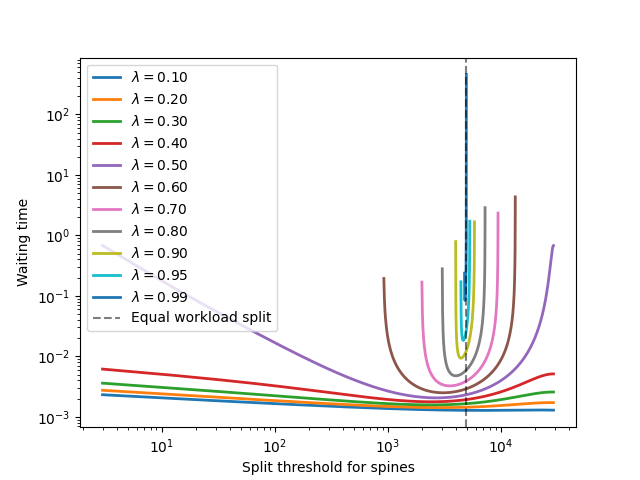
\includegraphics[width=.99\linewidth]{Chapter3/Figures/equal_workload_split_bpws}
		\caption{Optimal load balance threshold}
		\label{fig:cost-ws}
	\end{subfigure}%
	\begin{subfigure}{.5\textwidth}
		\centering
		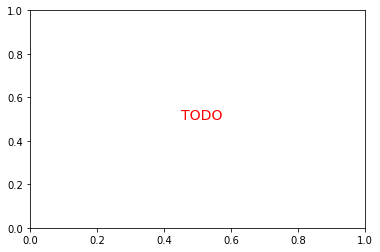
\includegraphics[width=.99\linewidth]{Chapter3/Figures/todored}%TODO change fig with the one with crossing lines
		\caption{Load distribution per-server }
		\label{fig:perspineload-ws}
	\end{subfigure}
	\caption{Web search workload. Simple case of $K$=2.}
	\label{fig:lbthreshold-ws}
\end{figure}
\\
\begin{figure}
	\centering
	\begin{subfigure}{.5\textwidth}
		\centering
		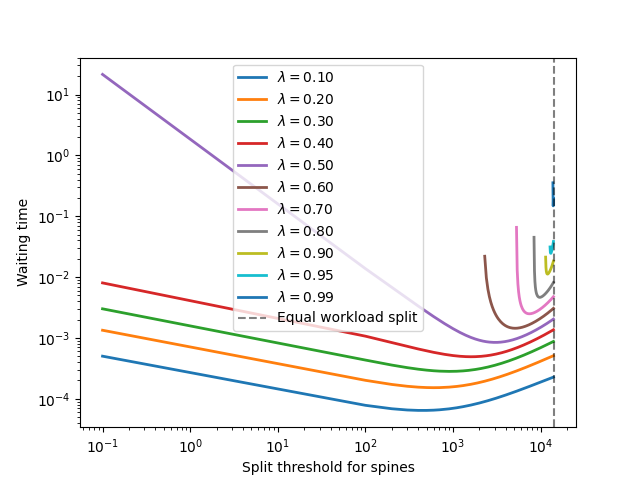
\includegraphics[width=.99\linewidth]{Chapter3/Figures/equal_workload_split_bpdm}
		\caption{Optimal load balance threshold}
		\label{fig:cost-dm}
	\end{subfigure}%
	\begin{subfigure}{.5\textwidth}
		\centering
		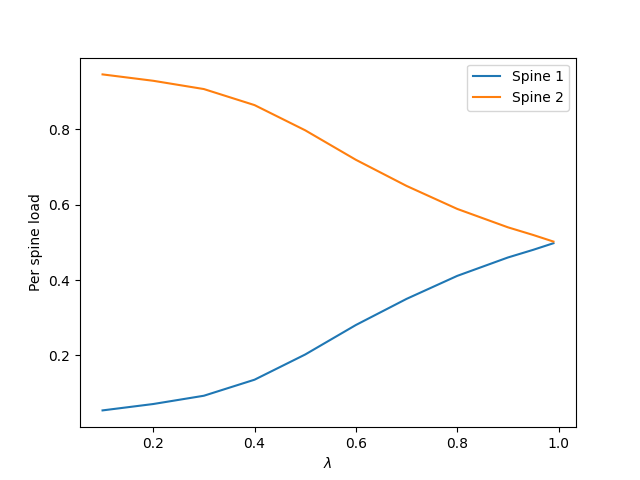
\includegraphics[width=.99\linewidth]{Chapter3/Figures/per_spine_load_bpdm}
		\caption{Load distribution per-server }
		\label{fig:perspineload-dm}
	\end{subfigure}
	\caption{Data mining workload. Simple case of $K$=2.}
	\label{fig:lbthreshold-dm}
\end{figure}%TODO per spine load measured or plugged threshold in equation? 
\subsubsection{Load balance on 2 parallel servers}
In the basic case of $K$=2 parallel servers, it is possible to plot the average sojourn time when varying the load balance threshold. Figures \ref{fig:cost-ws} and \ref{fig:cost-dm} show the aspect of the cost functions just described for the web search and the data mining workloads, respectively. All the axes are in log-scale and each curve represents a different normalized traffic $\lambda$. The vertical lines correspond the split that gives perfect load balance, apportioning half of the traffic on the high priority server and half on the low priority one. This split may be interchangeably referred to as \emph{perfect split} or \emph{proportionate split}. One phenomena is visible for both workloads, confirming previous intuitions. Imagine to connect the dots corresponding to the minima of the cost functions. The optimal load balance threshold does not coincide, broadly speaking, with the proportionate split threshold. Depending on the traffic level at which the system is operated and the workload, the optimal threshold triggers an earlier or later demotion with respect to the perfect split case. Equivalently, the jobs are distributed unfairly between the two servers (Figures \ref{fig:perspineload-ws}-\ref{fig:perspineload-dm}). For data mining, the imaginary line would be always in the leftmost side with respect to the proportionate split. That is, apart from loads close to saturation, the high priority server is kept as jobless as possible and the majority of work is sent to the low priority server. This result is coherent with the shape of the data mining workload, that presented huge variability. Plenty of short flows carrying few bytes are kept on a separated link from medium sized flows and a couple of long flows. This is not a surprise, since the problem formulation weighted more the average sojourn times of short flows. Slightly different trend is observed for web search. Moving from low to high values of $\lambda$, the optimal threshold is initially greater than the perfect split axis, then switches to its left and finally the two coincide. TODO Why??? For both cases, the objective function becomes much more extremely curled and steep around the perfect split axis when the load approaches the saturation value 1.  As already remarked, this is inevitable in order to fully exploit all the available capacity offered by the two parallel servers. At so high load any other traffic split would overload one of the two links and strongly deteriorate the average completion time of the flows going through it. Consistently, the cost function grows very rapidly in the neighborhood of the perfect split threshold value. \\
Finally, the two workloads have different sensitivities to the load balance threshold optimization. In particular, the web search achieves appreciable FCT gains starting from medium loads only ($\lambda > 0.5$) with (TODO provide some numbers), whereas at low loads there is no practical difference with the proportionate split. On the contrary, the data mining distribution gives theoretically a (TODO percentage) lower waiting time even for $\lambda$=0.1. This again reflects the extreme variability of the workload, that is comprised by a disproportionate number of short flows. The perfect split would keep a lot of mice flows mixed with low priority flows of bigger size for protracted service time. Instead, the optimal threshold reroute few flows but lot of traffic on the low priority server. In fact, for $\lambda$=0.1 the absolute value of the optimal threshold is an order of magnitude lower than the proportionate split threshold, however only a small fraction of flows fits into this gap. 

\subsubsection{Validity of the model}
Summarizing, the above discussion confirms that the web search traffic is harder than the data mining to cope with. This is the reason why in the following some results are shown exclusively for this workload. 
Next, it is consolidated the validity of the stochastic optimization model with numerical simulations, in particular it is shown the effective benefit of optimal load balancing. The underlying topology is again the simplest one, comprised of two parallel M/M/1 servers with no inner prioritization. The serving discipline is Processor Sharing (PS), implemented with a fluid model where parallel flows are served with equally subdivided bandwidth. 
The average normalized flow completion time (nFCT) has been considered as the primary evaluation metric.
\begin{tcolorbox}
	\textbf{nFCT}: Given a fixed data center topology and pair of source-destination servers, <$s$, $d$>, define $FCT_{opt}(x)$ as the FCT achieved by a flow of length $x$ originated from $s$ and directed to $d$ in a completely empty DCN. Let $FCT(x)$ as the FCT of a flow of length $x$ in a DCN in the presence of other flows. Let $X$ be the set of all possible flow lengths. Define:
	\[
	nFCT = \sum_{x \in X} \small \frac{FCT(x)}{FCT_{opt}(x)} \normalsize.
	\]
\end{tcolorbox}
The normalized flow completion time is very similar in spirit to the average slowdown presented in Sec.\ref{sec:las}, but it is more handful as it is dimensionless. Its advantage is to put all flows on the same comparable scale, permitting a clean visual analysis of fairness with respect to flow size. By the way, this kind of evaluation is important to us, as spatial diversity mainly targets short flows. \\
Figures \ref{fig:optlb-ws}-\ref{fig:optlb-dm} report the nFCT gain obtained thanks to the sole load balance optimizer. 
\begin{figure}
	\centering
	\begin{subfigure}{.5\textwidth}
		\centering
		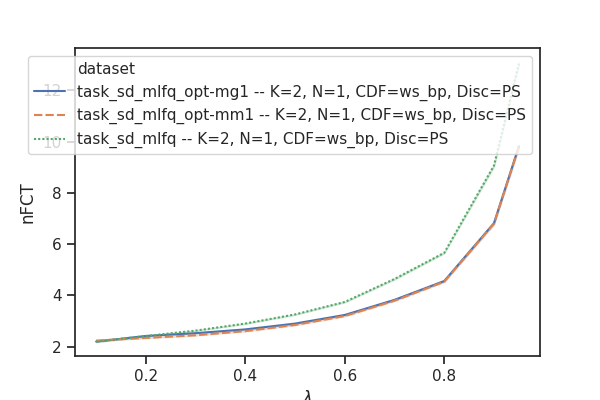
\includegraphics[width=1.05\textwidth]{Chapter3/Figures/ws_ps_comparison}
		\caption{nFCT comparison}
		\label{fig:optlbgain-ws}
	\end{subfigure}%
	\begin{subfigure}{.5\textwidth}
		\centering
		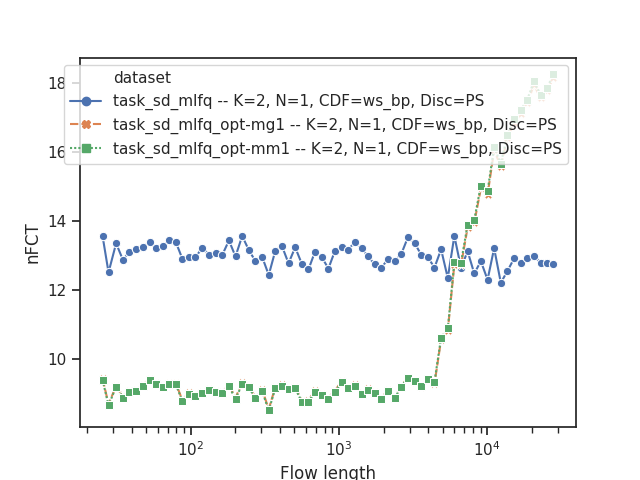
\includegraphics[width=\textwidth]{Chapter3/Figures/ws_ps_detailed.png}
		\caption{Per-flow length nFCT}
		\label{fig:optlbgainvsflowsize-ws}
	\end{subfigure}
	\caption{Web Search workload}
	\label{fig:optlb-ws}
\end{figure}
\begin{figure}
	\centering
	\begin{subfigure}{.5\textwidth}
		\centering
		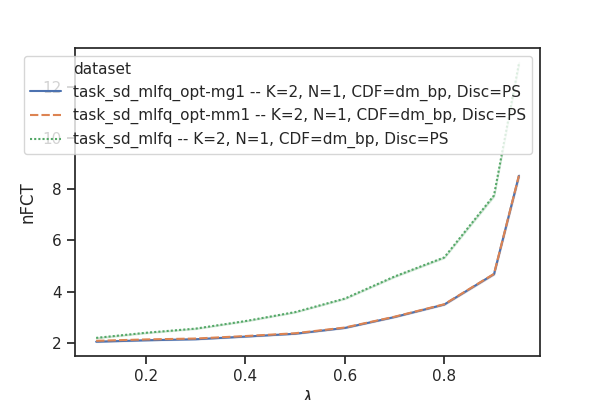
\includegraphics[width=1.05\textwidth]{Chapter3/Figures/dm_ps_comparison.png}
		\caption{nFCT comparison}
		\label{fig:optlbgain-dm}
	\end{subfigure}%
	\begin{subfigure}{.5\textwidth}
		\centering
		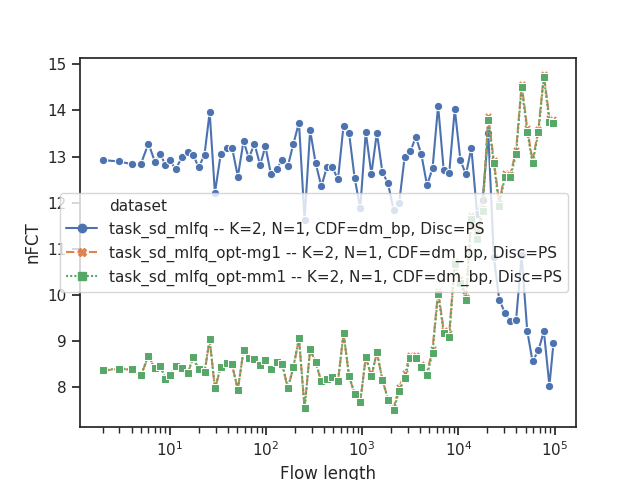
\includegraphics[width=\textwidth]{Chapter3/Figures/dm_ps_detailed.png}
		\caption{Per-flow length nFCT}
		\label{fig:optlbgainvsflowsize-dm}
	\end{subfigure}
	\caption{Data Mining workload}
	\label{fig:optlb-dm}
\end{figure}
Two ( TODO three if we talk about M/G/1 ) different scenarios are compared. Both adopt spatially-diverse MLFQ, but in one case the load balance threshold is optimized, in the other not. The former case is labeled as \texttt{SD-MLFQ-OPT}, whereas the latter as \texttt{SD-MLFQ}. Call $s_0$ and $s_1$ the two servers (i.e links/queues) and $\Omega$ the unique demotion threshold. Newly arrived flows always enter the system through $s_0$ as their attained service equals to 0, then they are rerouted to the link $s_1$ when $s_0$ has transmitted $\Omega$ of their bytes. As expected, the benefits on the average completion times are more pronounced for the data mining distribution, at all loads (Figures \ref{fig:optlbgain-ws}-\ref{fig:optlbgain-dm}). Even so, appealing phenomena emerge when looking at the detailed breakdown of the response time versus flow size (Fig.\ref{fig:optlbgainvsflowsize-ws}-\ref{fig:optlbgainvsflowsize-dm}). First focus on the SD-MLFQ system without load balancing optimization and compare the blue curves. In web search, the normalized response time curve exhibits a constant plateau which testify a substantial invariance of the slowdown with respect to the flow length. Conversely, in data mining there is an abrupt transition to lower response times for flows longer than 20MB, which roughly corresponds to the demotion threshold adopted in this case. The difference is justified by the fact that the proportionate split threshold for data mining cuts the flow size CDF near the 99-th percentile, due to the oft-repeated heavy-tail characteristic of this workload. Therefore, only few long flows remain to share the processor of the low-priority server $s_1$ --- keep in mind that all servers have PS. Since the normalized FCT captures the slowdown in respect to the ideal case where the flow is serviced alone, it is explained such a behavior. Next, let's concentrate on the spatial diversity with optimal load balancing (green curves), which is the real goal to validate the model. The two workload perform similarly and have analogous trends. Specifically, the encouraging result is that shorter flows indeed take advantage of spatial diversity, as they are sent through a less loaded path. The opposite happens to long jobs, which undergone the dual effect.
%TODO at which lambda are these plots???
% TODO definition of main spatial diversity principles (bullet item list)
% TODO M/M/1 vs M/G/1 how implemented in practise? Assumed poisson arrivals but not true....what changed? How determined the variance of the job for subsequent servers? 
%TODO missing factor 2
\subsubsection{Analysis of the model scalability}
So far the only scenario that has been investigated is the simple case of two parallel servers without sub-thresholds. This was useful to get confident with the relationships between load balance and the spatial diversity demotion mechanism. However, in the more general setting there might be much more parallel servers and at least two priority levels per server. The total number of thresholds was reduced by decoupling the load distribution by the server-local prioritization. Thus, the total complexity only depends on the number of servers $K$. Unfortunately, it is still typically high. 
% dire python scipy solver
% citare basin hoppin e pso heuristics (some parameters used, bla bla)
% TODO why complexity is higher at load 0.6 ???
\subsection{Finding sub-thresholds}
\label{sec:subthresh-with-sd}
Lastly, it is addressed the problem of finding the sub-thresholds. Starting from the optimal load balance thresholds that have been found with the solver, each server is then treated individually. In other words, the demotion from one server to another with the optimal load balance split makes each server observe a different version of the initial workload. Indeed, subsequent servers receive only flows larger than the precedent demotion thresholds, thus they handle truncations of the original flow size distribution above increasing percentiles. A clarifying overview is provided in Fig. \ref{fig:sd-spine-distribution} for the case of $K$=3 servers $s_0$, $s_1$, $s_2$. As usual, lower indexes identify higher priorities. Figure \ref{fig:wsbp-cdf} is the web search flow size distribution, from which new jobs are randomly generated. In a data center network, this would be the DC-wide workload. On the same axes are drawn the two optimal split thresholds, denoting the amount of service in kilobytes after which a flow is rerouted from $s_0$ to $s_1$ and then from $s_1$ to $s_2$. Call these thresholds $\Omega_1$ and $\Omega_2$ respectively. 
\begin{figure}
	\centering
	\captionsetup{width=.8\linewidth}
	\begin{subfigure}{.3\textwidth}
		\centering
		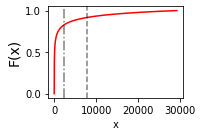
\includegraphics[width=1.05\textwidth]{Chapter3/Figures/ws-bp-cdf}
		\caption{Workload on $s_0$}
		\label{fig:wsbp-cdf}
	\end{subfigure}%
	\hfill
	\begin{subfigure}{.3\textwidth}
		\centering
		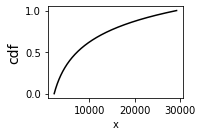
\includegraphics[width=\textwidth]{Chapter3/Figures/wsbp-highp-cdf}
		\caption{Workload on $s_1$}
		\label{fig:highp-cdf}
	\end{subfigure}
	\hfill
	\begin{subfigure}{.3\textwidth}
	\centering
	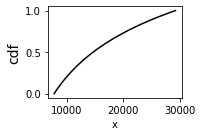
\includegraphics[width=\textwidth]{Chapter3/Figures/wsbp-lowp-cdf}
	\caption{Workload on $s_2$}
	\label{fig:lowp-cdf}
	\end{subfigure}
	\caption{Job size distributions observed by servers $s_0$, $s_1$, $s_2$ in decreasing order of priority. Optimal load balance split for $\lambda=0.9$.}
	\label{fig:sd-spine-distribution}
\end{figure}
Since all flows enter the system through $s_0$, this distribution is also the one observed by the highest priority server. Keep in mind that this is just the distribution to which a job belongs and not the actual traffic handled by a server. Indeed, $s_0$ serve only the first $\Omega_1$ bytes of these flows. The byte arrivals were obtained with Eq.\eqref{load-on-pqi}, that does require this distribution to be known. Then, subsequent servers of lower priorities observe left-truncated versions of the initial workload on $s_0$. These p.d.f. $f(x)$ and the corresponding c.d.f. $F(x)$ (Fig.\ref{fig:highp-cdf}-\ref{fig:lowp-cdf}) can be written as distribution conditioned to the new support $[\Omega_{s-1},\infty)$:
\begin{equation}
\label{eq:conditionalpdf}
\begin{aligned}
F(x|x>\Omega_{s-1}) &= \dfrac{F(x) - F(\Omega_{s-1})}{1-F(\Omega_{s-1})}  \\
f(x|x>\Omega_{s-1}) &= \dfrac{f(x)}{1-F(\Omega_{s-1})} 
\end{aligned}
\end{equation}
Nicely, these scaled distributions are still bounded Pareto, thanks to the scale-invariance property of this family of distributions. However, notice that their heavy-tails are progressively reduced with strong implications in limiting the applicability of spatial diversity to very large topologies. More details on this will be provided in the remaining of this work. \\
Once these distributions are known, nothing is missing to apply the greedy sub-threshold assignment algorithms depicted in Sec. \ref{sec:greedy-thresh}. For completeness, they are briefly rewritten under this framework. Define in short:
\begin{align*}
	f_T(x) =& f(x|x>\Omega_{s-1})\\
	\bar{F}_T(x) =& \bar{F}(x|x>\Omega_{s-1}). 
\end{align*}
Enumerate the available server $s \in \{1,..,K\}$. The goal is to find on all servers a set of sub-thresholds $\alpha_i^s$ to delimit demotion bounds across priority queues $i \in \{1,..,N\}$. \\
\textit{Equal-Split-N} (ES-N) is substantially the same:
\begin{equation}
\alpha_i^s = F_T^{-1}\Big(\frac{i}{N}\Big)
\end{equation}
\textit{Load-Split-N} (LS-N) is also very similar. It required the solution of the set of load balance equations \ref{eq:main-K-PQ}. The expression of the average traffic $\mathbb{E}[L_i^s]$ on priority $i$ of server $s$ is unchanged. However, additional care must be paid to their sum $\sum_{i=1}^{N}\mathbb{E}[L_i^s]$. From proof \ref{proof}, this sum was equal to:
\[
\sum_{i=1}^{N}\mathbb{E}[L_i^s] = \int_{\Omega_{s-1}}^{\Omega_s}xf_T(x)dx + \Omega_{s} \bar{F}_T(\Omega_{s}) -\Omega_{s-1}\bar{F}_T(\Omega_{s-1})
\]
and the terms outside the integral always amounted to zero, so that the sum gave $\int_{\Omega_{s-1}}^{\Omega_s}xf_T(x)dx = \mathbb{E}[X]$. Instead, in this case they are generally different zero because the lower threshold $\alpha_0^s = \Omega_{s-1} \neq 0$ and the survival function above the upper threshold $\bar{F}_T(\alpha_N^s) = \bar{F}_T(\Omega_s) \neq 0$. Everything else is the same.
\\

As already mentioned, it is very likely that this approach is sub-optimal. However, it represents an handful way of computing all the thresholds in order to establish some understanding about the integration of spatial diversity with an MLFQ system. The next section will be an in-depth analysis of such dynamics, increasing the dimensionality of the system both in the number of servers and in the number of priorities.

\section{The service discipline: FIFO or PS?}
In the previous section it was laid down the basic framework of spatial diversity. It was remarked the fact that adopting spatial diversity translates into a priority-driven load balancing. At the same time were collected encouraging results about the effectiveness of the optimal load balancing. It was discussed the impact of two workloads commonly used as a benchmark in literature. Then, it was solved the optimal load balancing problem for up to $K$=9 parallel servers and explained how to compute the sub-thresholds without trying to face the overwhelming complexity of the optimal approach. In all the simple experiments carried out, the servers were always configured with Processor Sharing service discipline and without priority queues.

This section aims to provide answers to principally two things. The first one is the behavior of the priority-driven load balancing when increasing the number of server $K$ up to 9 parallel servers. Second, it is treated the integration of the priority-driven load balancing with the legacy MLFQ system. In practice, it is considered the general case where each server has many PQs on its interfaces used in strict priority. As it will be explained shortly, it turns out that for both attempts, the performances of the system are highly correlated with the adopted servicing policy. Considered cases are the FIFO (FCFS) servers and the usual PS servers. 

\subsection{Dimensioning spatial-diversity}
\label{sec:dimensioning-spatial}
First it is addressed the first question: what are the effects of augmenting the spatial diversity \emph{rank}? 
\begin{tcolorbox}
	\textbf{SD-rank}: Given a data center topology with $S$ spines --- or the equivalent system of parallel M/M/1 servers where is applied priority-driven load balancing, that is each server handle a group of priority and a flow is routed depending on its assigned priority. Let's define the spatial-diversity rank (SD-rank) as the number $K$ of servers which handle different priorities. 
\end{tcolorbox}
The spatial diversity ranks tells how many M/M/1 servers (or group of servers) are considered to be used to implement spatial diversity. For example, suppose there are 4 parallel servers available $s_0$, $s_1$, $s_2$, $s_3$. Consider these two possibilities. 
\begin{enumerate}
	\item \textbf{Rank 2}. The four servers are grouped in two pairs, say $(s_0, s_1), (s_2,s_3)$. Spatial diversity demotion is applied at pair level. This means there is only one load balance threshold $\Omega$. When the longest flow enters the system, it is sent at random either on $s_0$ or $s_1$. As soon as the flow has received service $\Omega$ it is demoted, again randomly, either on $s_3$ or $s_4$. In other words, this can be seen as a system of only two parallel servers with twice the capacity each, where only one rerouting happens to the longest flow. 
	\item \textbf{Rank 4 \textit{(full-rank)}}. The servers are not grouped in any way. All servers participate to the priority-driven load balance. Therefore, there are 3 thresholds and the longest flow it is rerouted three times.
\end{enumerate}
In the next experiments (Fig.\ref{fig:lb-var-K-fifo}) is evaluated the full-rank spatial diversity system for three topologies, corresponding to $K=3$, $K=5$, $K=9$ and for two serving policies: PS and FIFO. The number of priority queues $N$ is still one per server. Remember that the numerical simulator is a job level simulator, thus flows are not fragmented in packets anyhow. This means that the FIFO policy is absolutely non-preemptive for jobs in the same priority queue. The service of a flow cannot be interrupted and flows arriving in the meanwhile are queued back in a first-in first-out order. Instead, the PS discipline subdivides the available capacity among all flows present in the system with a fluid approximation. Thus, a fresh flow share immediately the service rate granted to its priority queue with other flows in the same queue. 
\begin{figure}
	\centering
	\begin{subfigure}{.5\textwidth}
		\centering
		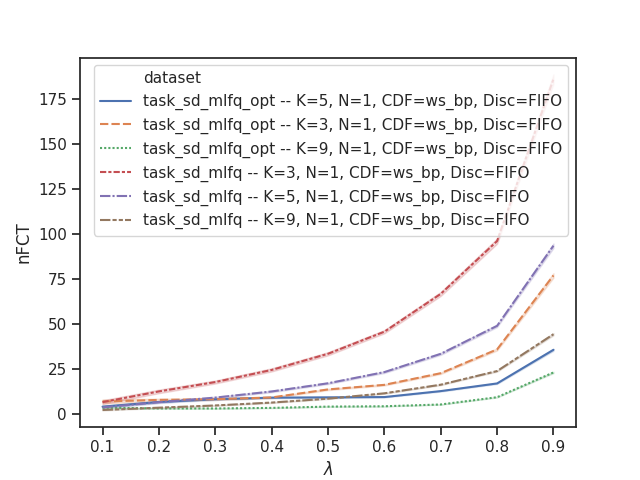
\includegraphics[width=0.99\textwidth]{Chapter3/Figures/lb_opt_vs_nopt_comparison}
		\caption{nFCT comparison}
	\end{subfigure}%
	\hfill
	\begin{subfigure}{.5\textwidth}
		\centering
		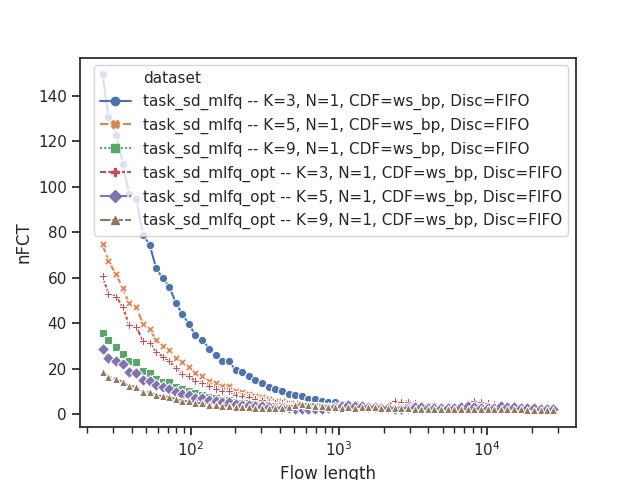
\includegraphics[width=0.99\textwidth]{Chapter3/Figures/lb_opt_vs_nopt_detailed}
		\caption{Per-flow length nFCT ($\lambda$=0.9)}
		\label{fig:lb-var-K-fifo-detailed}
	\end{subfigure}
	\caption{Web Search workload and FIFO discipline at 99\% confidence interval.}
	\label{fig:lb-var-K-fifo}
\end{figure}
\begin{figure}
	\centering
	\begin{subfigure}{.5\textwidth}
		\centering
		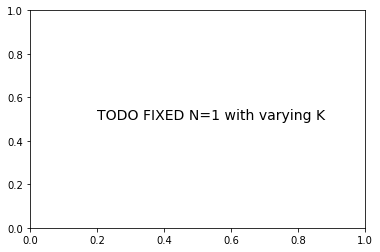
\includegraphics[width=0.99\textwidth]{Chapter3/Figures/todo}
		\caption{nFCT comparison}
	\end{subfigure}%
	\hfill
	\begin{subfigure}{.5\textwidth}
		\centering
		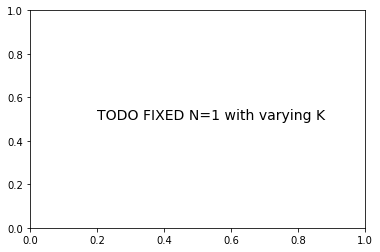
\includegraphics[width=0.99\textwidth]{Chapter3/Figures/todo}
		\caption{Per-flow length nFCT ($\lambda$=0.9)}
		\label{fig:lb-var-K-ps-detailed}
	\end{subfigure}
	\caption{Web Search workload and PS discipline at 99\% confidence interval. \textcolor{red}{GRAFICI MANCANTI MA SIMULAZIONI GERMAN CON QUELLO SCENARIO GIA FATTE MA USATE NEI GRAFICI FINALI. CHIEDERE GRAFICO A PARTE SE UTILE}}
	\label{fig:lb-var-K-ps}
\end{figure}
%TODO Processor Sharing for fixed N=1 and varying K
%TODO when N=2 and FIFO what's the policy?
These experiments were carried out both with and without the optimized load balance thresholds. The first very positive observation is that, whatever the number of servers, the optimal load balance wins over the proportionate split. This again confirms the validity of the queuing model formulation for load balancing. 
The FIFO policy is clearly unfair with respect to short flows (Fig.\ref{fig:lb-var-K-fifo-detailed}). This is because without preemption a single elephant flow could starve a myriad of short flows. The unfairness is mitigated when increasing the spatial diversity rank, as long flows are demoted earlier and leave quickly high priority servers. Notably, for a fixed $K$, having $N$=1 priority queue is the worst case from the point of view of mice flow starvation. With $N$>1 PQs, the service received by a flow on each server would be broken in multiple phases, each on a different priority queue. Since the PQs are scheduled in Strict Priority order and newly arrived flows enter in high priority, a short flow behind longer ones would have to wait only until the demotion at lower priority of the flows ahead. Somehow the demotion preempts the long flows, and weaken the impact of having a FIFO policy on the PQs themselves. The scenario changes with the PS service discipline. Short flows do not suffer the same issues yet mentioned, because they always share the processor with other flows. However, when increasing the rank long flows start to be excessively penalized. Remember that subsequent servers observe cut workloads, whose heavy-tailed property is gradually destroyed. In other words, the flow size distributions fed in low priority servers have reduced variability (Fig. \ref{fig:cdfs}). This is a clear downside for PS policy. Indeed, it is well-known that under the assumption of low variability of the distribution, it is better to adopt a FCFS order. As a trivial example, suppose to schedule two flows $f_1, f_2$ of size 10 bits/bytes/packets,... Denote as $T(f_i)$ the average flow completion time of flow $i$, expressed in transmission slots. FIFO scheduling would give:
\[
	T_{FIFO}(f_1) = T_{FIFO}(f_2) = \dfrac{10+20}{2} = 15
\]
Instead, PS scheduling would be worse:
\[
T_{PS}(f_1) = T_{PS}(f_2) = \dfrac{19+20}{2} = 19.5
\]
\textcolor{red}{TODO PRECEDENTE DISCORSO VA VERIFICATO CON IL GRAFICO SOPRA MANCANTE}\\
The study of the system with increased number of priority queues led to even more surprising results. This step really integrates the spatial diversity in the legacy MLFQ system with many priority levels. Here it is reported only the Processor Sharing discipline for the reasons explained few lines above. It is clear that for the FIFO case increasing $N$ further minimize the average flow completion time. A simulative result confirming this fact will be present in the last section \S \ref{sec:final-comparison} of the chapter during the final comparisons of SD-MLFQ (spatial diversity case) with ES-N (non spatial diversity case). Figure \ref{fig:sdmlfq-variable-N} is a key result that will uncover potential bottlenecks of SD-MLFQ. In this experiments are compared the average flow completion times of the system with fixed $K$=4 and variable $N$. Load balance thresholds are not optimized in this case, but are set to grant the proportionate split of the traffic on the four parallel servers. The sub-thresholds have been assigned with the simple ES-N variation for spatial diversity (\S \ref{sec:subthresh-with-sd}). Very interestingly, this numerical results provide a different perspective on the ideal granularity of priority queues per server with respect to previous works. While on the systems that approximate LAS or SRPT schedulers with PQs  \cite{pias, pFabric}, increasing the number of priority queues is always beneficial, it is not so when spatial diversity is introduced. At low load there is not a visible difference among the simulated scenarios. However, at high load the best average nFCT is attained with $N$=2 priorities per server (dashed orange curve). The peculiar phenomenon is the behavior of the case $N$=8 (red curve), whose corresponding nFCT starts to increase consistently above $\lambda=0.8$. 
\begin{figure}
	\centering
	\begin{subfigure}{.5\textwidth}
		\centering
		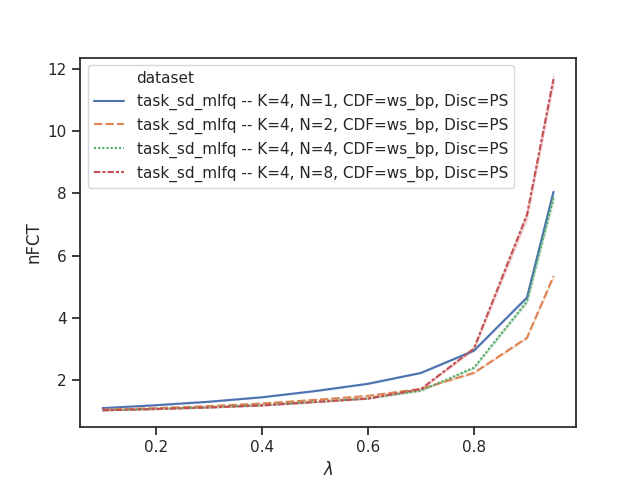
\includegraphics[width=0.99\textwidth]{Chapter3/Figures/sd_mlfq_k4_comparison.png}
		\caption{nFCT comparison}
		\label{fig:sdmlfq-variable-N-fct}
	\end{subfigure}%
	\hfill
	\begin{subfigure}{.5\textwidth}
		\centering
		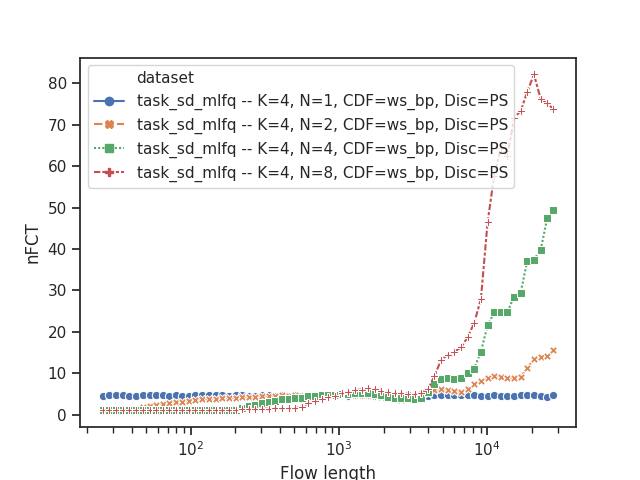
\includegraphics[width=0.99\textwidth]{Chapter3/Figures/sd_mlfq_k4_detailed.png}
		\caption{Per-flow length nFCT ($\lambda$=0.9)}
		\label{fig:sdmlfq-variable-N-fct-detailed}
	\end{subfigure}
	\caption{Web search workload and PS discipline at 99\% confidence interval}
	\label{fig:sdmlfq-variable-N}
\end{figure}
From the detailed breakdown of Fig.\ref{fig:sdmlfq-variable-N-fct-detailed}, it is evinced that the most severe degradation happens to long flows. They suffer an unacceptable penalty, which globally makes also the average worse. As a general trend, an higher number of priorities per server is reflected in a more pronounced raise of the job response time of long flows. At the same time, coherently with the scheduling theory of LAS (\S \ref{sec:las}) and the results of PIAS, flows between 100KB and 1MB (medium size flows) are improved. \\ \\
Such an extreme behavior on long flows was worth of extra-attention. In particular, it brings up an important question: is the best choice to configure low priority servers with a fine-grained prioritization?
\subsubsection{Elephant demotion}
\textcolor{red}{TODO Describe figures of hazard rate and optimal demotions for low priority spines. Link this observation with previous intuition that subsequent spines observe distribtions with less and less variability (LAS and SRPT require high variability !!!)}. 
\subsubsection{Flow synchronization}
\textcolor{red}{Problems of previous subsubsection are exacerbated by flow syn phenomenon (not observed in PIAS)}.
\subsection{Final comparison}
\textcolor{red}{Final comparison with ES-N (no spatial). Show plots and resume table}.
